\section{基于RISC-V64的NPUcore内核运行}
\subsection{星光二代开发板简介}
\textbf{昉·星光 2 简介}

\begin{figure}[ht]
	\centering
	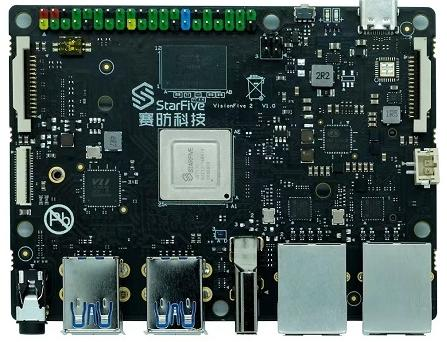
\includegraphics[width=0.5\linewidth]{figures/08-02-昉·星光 2.jpg}
	\caption{昉·星光 2}
\end{figure}

昉·星光 2 是一款集成了GPU的高性能RISC-V单板计算机。它搭载四核64位RV64GC ISA的芯片平台(SoC),工作频率最高可达1.5 GHz,开源的昉·星光 2具有强大的软件适配性,官方适配Debian操作系统,同时通过社区合作适配各种Linux发行版,包括Ubuntu、OpenSUSE、OpenKylin、OpenEuler、Deepin等,及在这些操作系统上运行的各类软件。接下来我们的上板实验就在昉·星光 2 上进行。

\textbf{硬件准备}

在进行上板实验前,首先需要准备以下硬件设备:

{
	\ding{172} 昉·星光 2 开发板
	
	\centering
	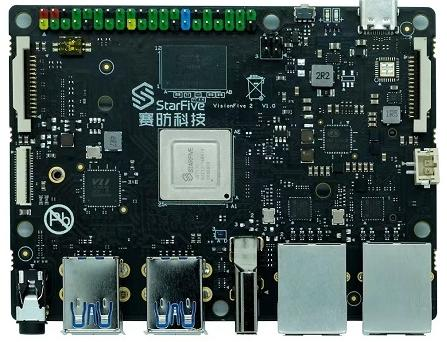
\includegraphics[width=0.5\linewidth]{figures/08-02-昉·星光 2.jpg}
	
	\raggedright
	\setlength{\parindent}{2em}
	\ding{173} 开发板充电线(type-c 充电线)
	
	\centering
	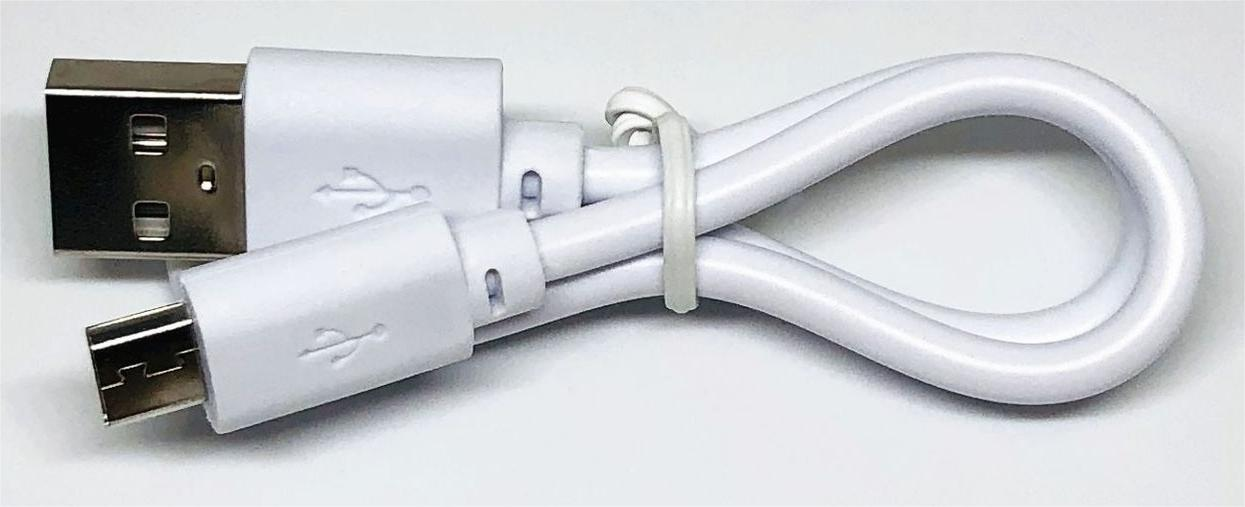
\includegraphics[width=0.5\linewidth]{figures/08-02-开发板充电线.jpg}
	
	\raggedright
	\setlength{\parindent}{2em}
	\ding{174} USB TO TTL串口通信转化器
	
	\centering
	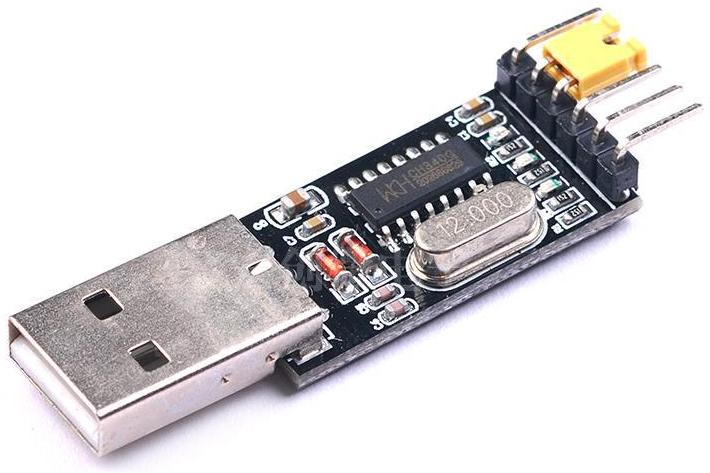
\includegraphics[width=0.5\linewidth]{figures/08-02-USB TO TTL 串口通信转化器.jpg}
	
	\raggedright
	\setlength{\parindent}{2em}
	\ding{175} 母对母杜邦线
	
	\centering
	
\includegraphics[width=0.5\linewidth]{figures/08-02-杜邦线.jpg}
	
	\raggedright
	\setlength{\parindent}{2em}
	\ding{176} RJ45 网线
	
	\centering
	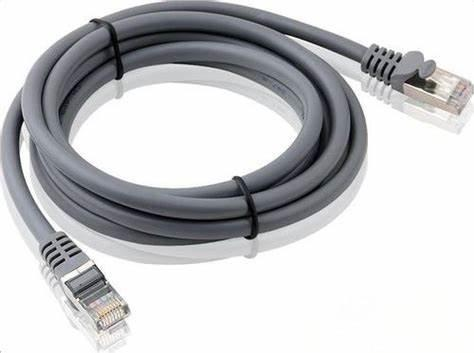
\includegraphics[width=0.5\linewidth]{figures/08-03-RJ45网线.jpg}
	
	\raggedright
	\setlength{\parindent}{2em}
	\ding{177} 拓展坞
	
	\centering
	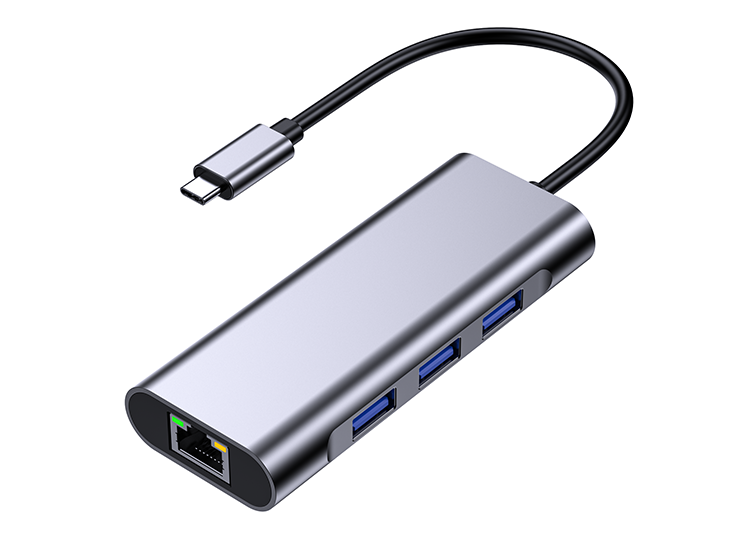
\includegraphics[width=0.5\linewidth]{figures/08-02-拓展坞.jpg}
	
	\raggedright
	\setlength{\parindent}{2em}
	拓展坞需要带至少一个网线接口,两个USB接口。如果笔记本电脑自带网线接口,并且电脑上的两个USB接口都空闲则不需要该拓展坞。
}

\textbf{昉·星光 2 引脚介绍}

查阅星光二代官网手册,得到星光二代引脚分布如图所示,
\begin{figure}[ht]
	\centering
	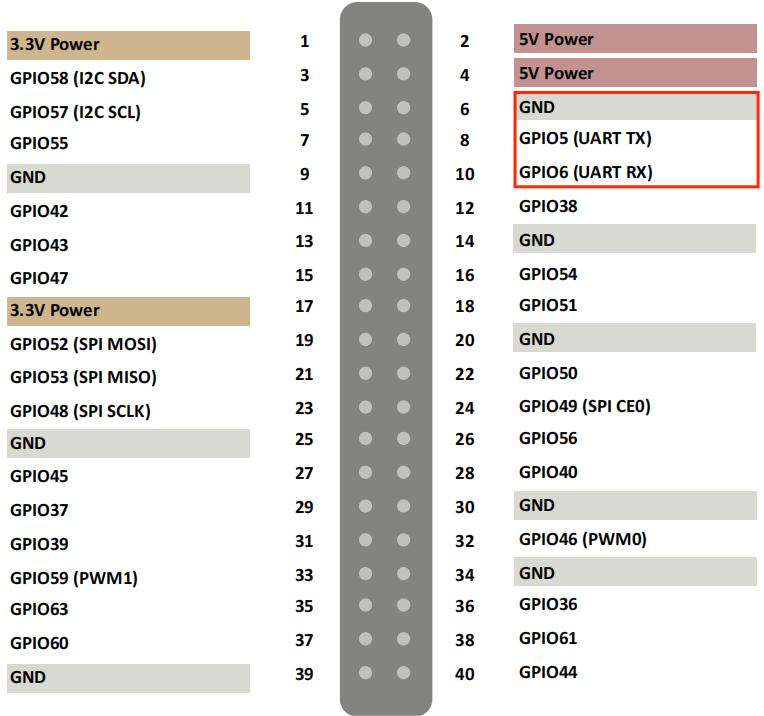
\includegraphics[width=0.8\textwidth]{figures/08-02-星光二代pin图.jpg}
	\caption{星光二代pin图}
\end{figure}

我们只需要进行串口连接,因此只需要关注红框内的 GND,UART TX,UART RX 串口即可,即图中的6、8、10号接口。

\textbf{硬件连接}

{
	\ding{172} 串口连接
	
	\raggedright
	\setlength{\parindent}{2em}
	首先,使用杜邦线连接串口通信转换器的TXD,RXD,GND 接口,仅连接这三个接口即可,剩余悬空,如下图所示。
	
	\centering
	\includegraphics[width=0.58\linewidth]{figures/08-02-杜邦线连接串口转换器.jpg}
	
	\raggedright
	\setlength{\parindent}{2em}
	
	然后,使用杜邦线连接昉·星光 2 单板计算机,连接到图中序号\ding{175}的引脚处。
	
	
	\centering
	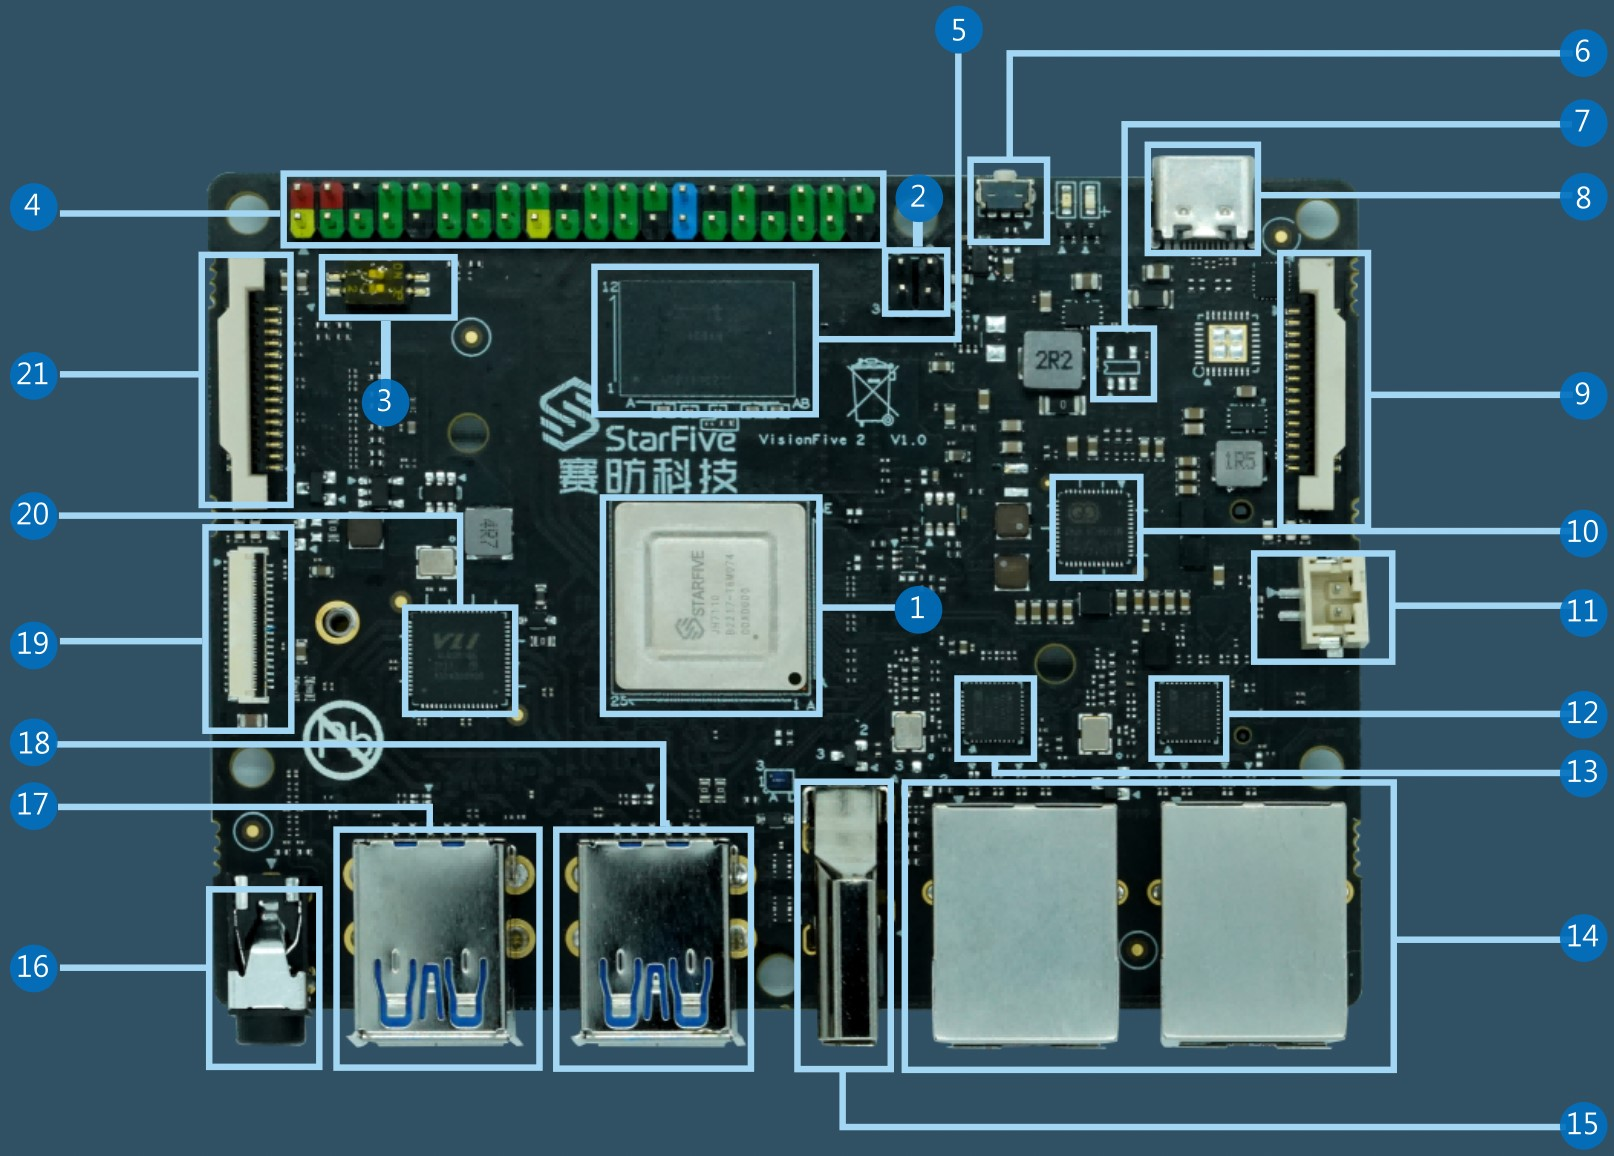
\includegraphics[width=0.58\linewidth]{figures/08-02-赛昉结构.jpg}
	
	\raggedright
	\setlength{\parindent}{2em}
	
	连接好后如下图所示
	
	\centering
	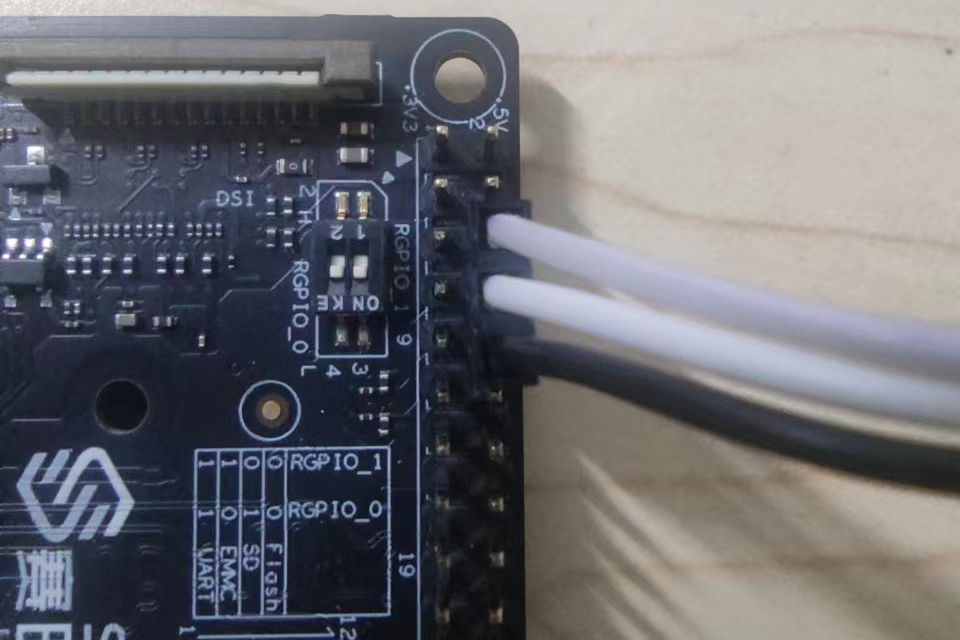
\includegraphics[width=0.58\linewidth]{figures/08-02-杜邦线连接赛昉.jpg}
	
	\raggedright
	\setlength{\parindent}{2em}
	
	\ding{173} 电源连接
	
	将电源线的 type-c 接口接入到图中插口\ding{179}处即可
	
	\centering
	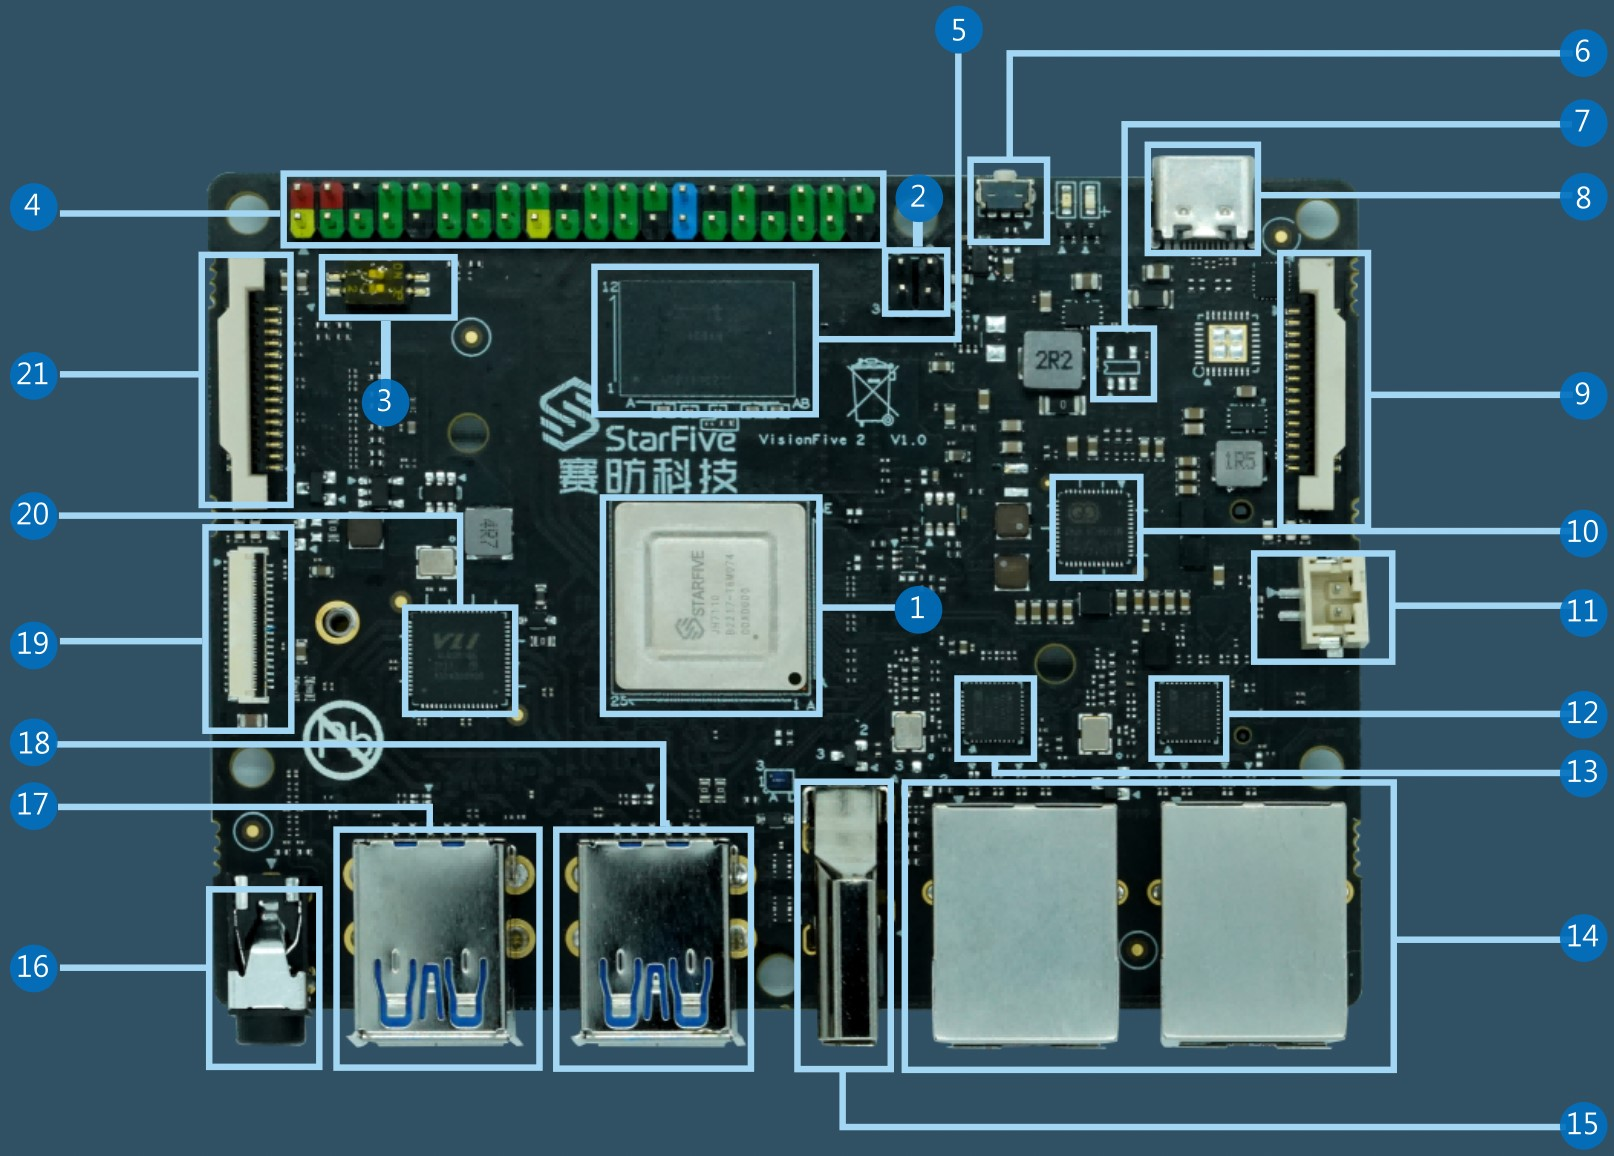
\includegraphics[width=0.58\linewidth]{figures/08-02-赛昉结构.jpg}
	
	\raggedright
	\setlength{\parindent}{2em}
	
	连接好后如下图所示
	
	\centering
	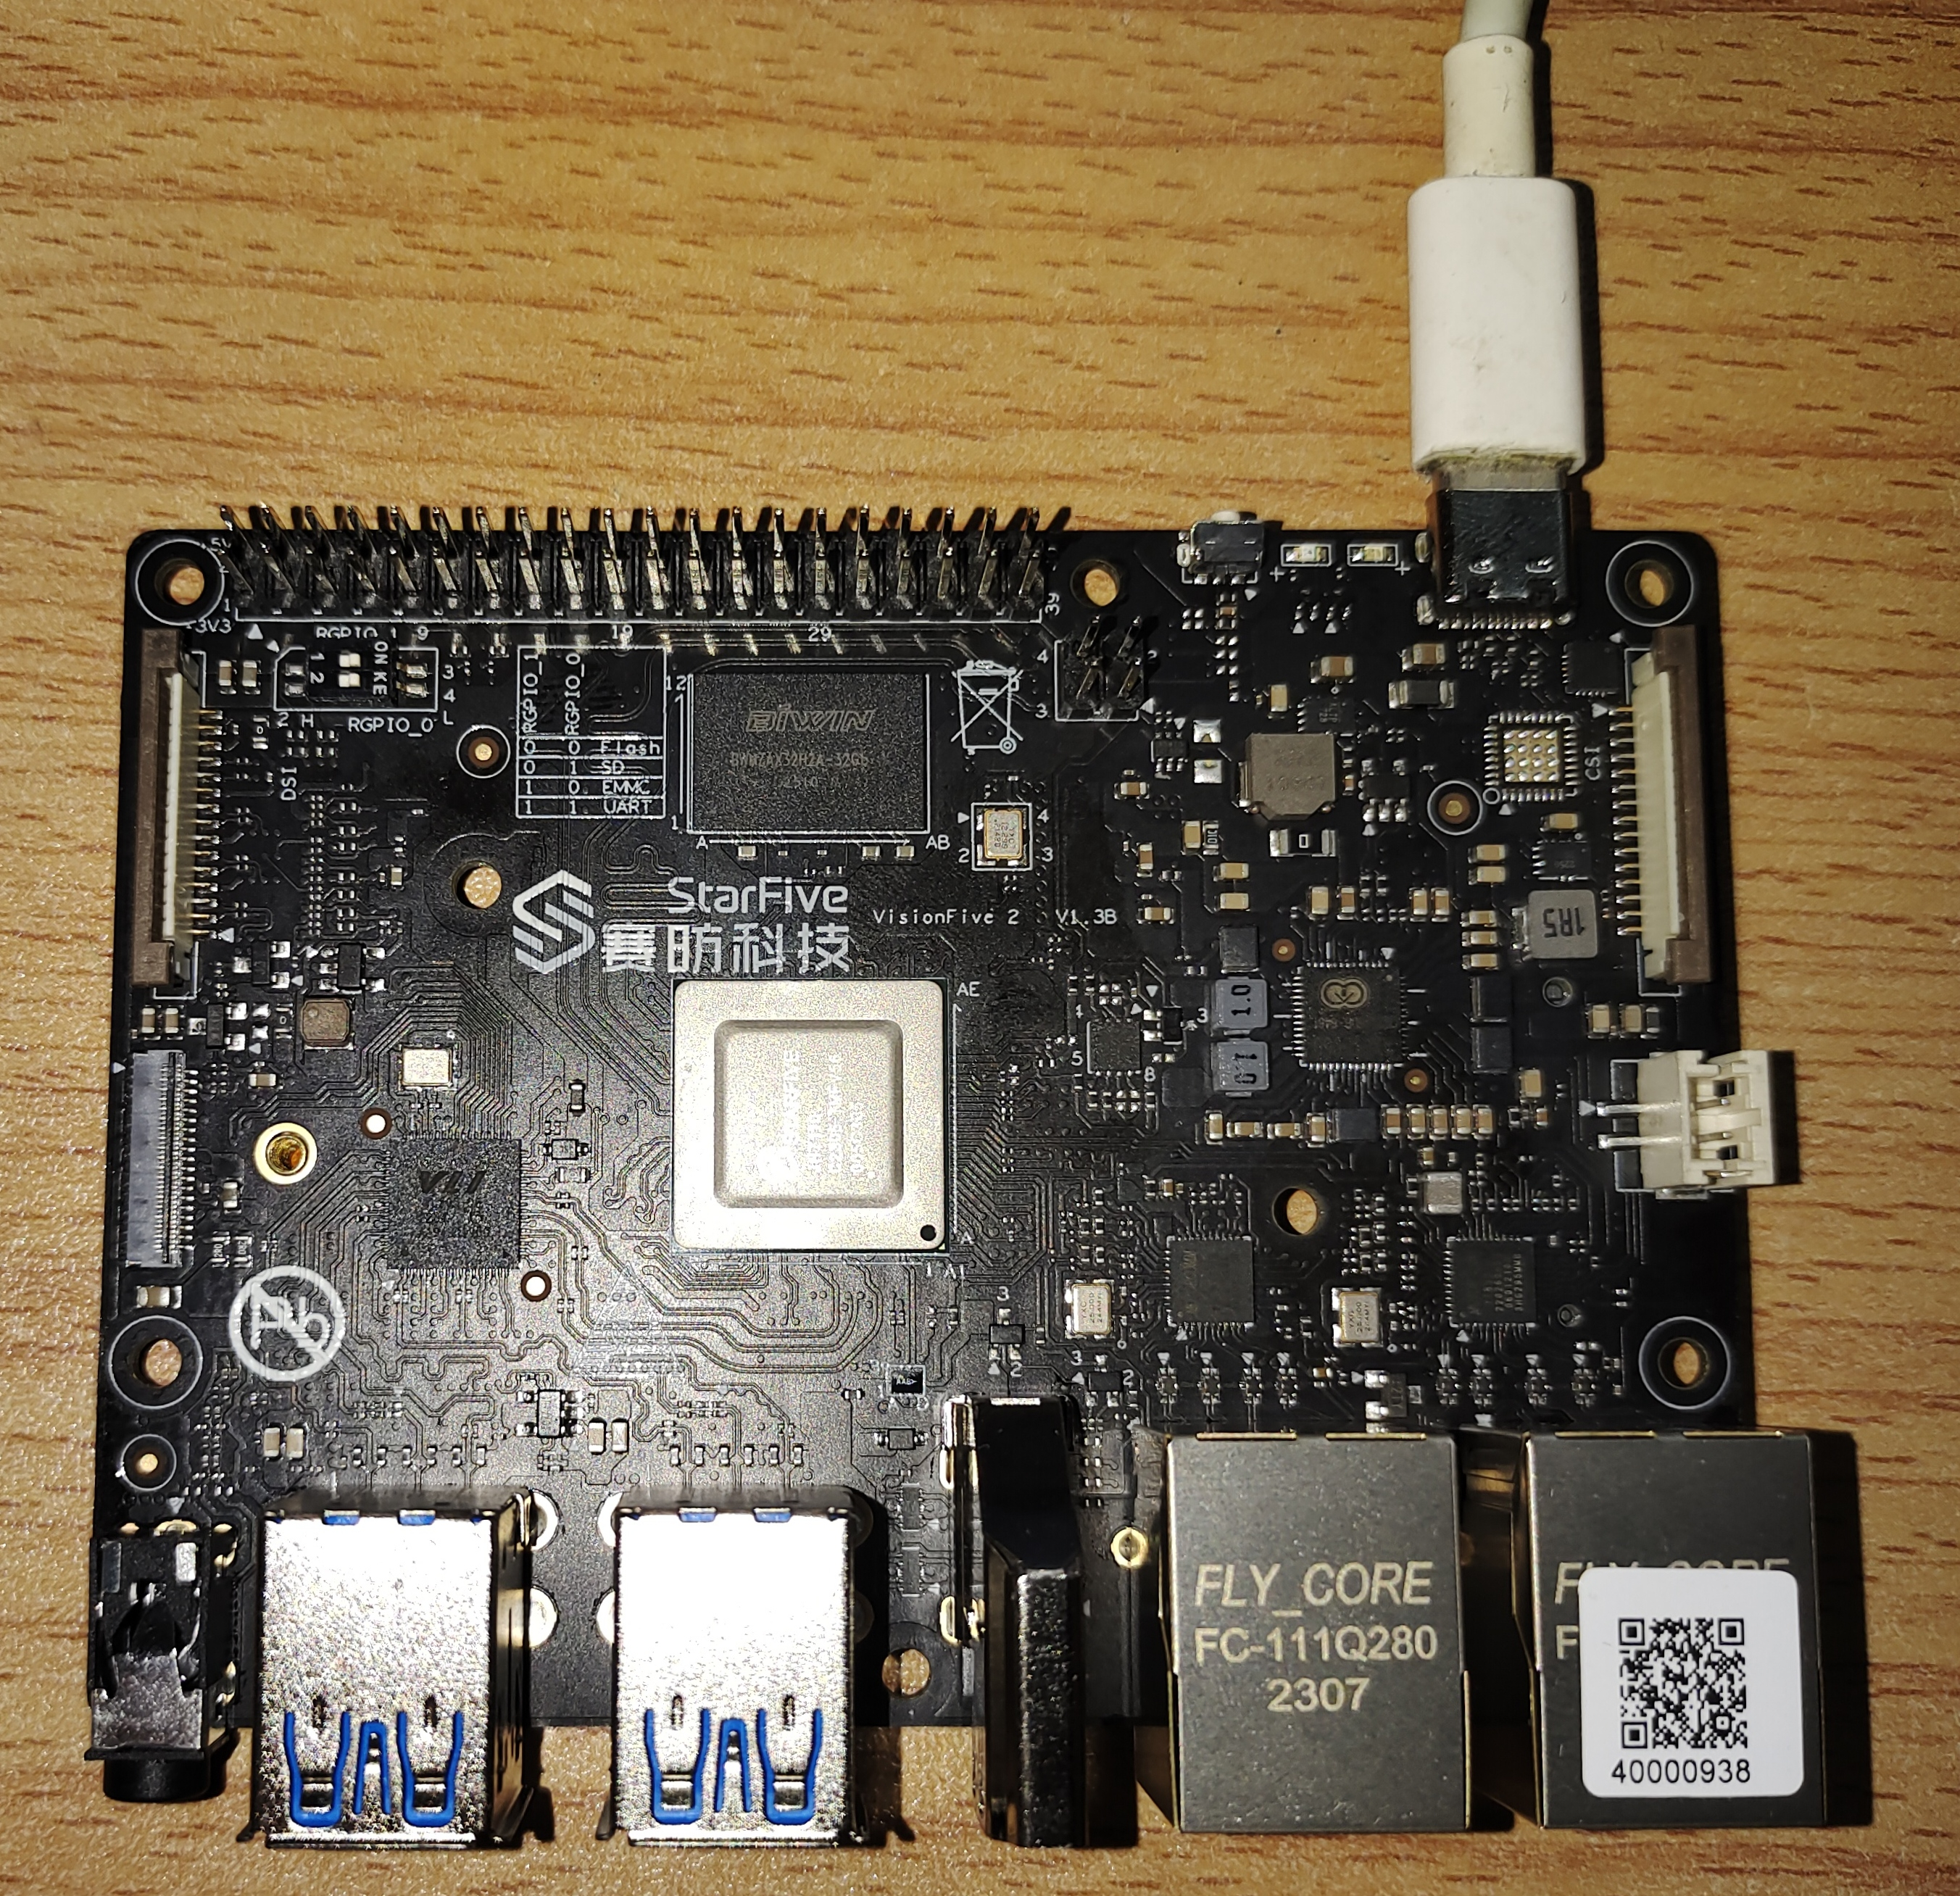
\includegraphics[width=0.58\linewidth]{figures/08-02-连接电源线.jpg}
	
	\raggedright
	\setlength{\parindent}{2em}
	\ding{172} 网线连接
	
	将电源线的 type-c 接口接入到图中插口\ding{185}处的任一插口即可
	
	\centering
	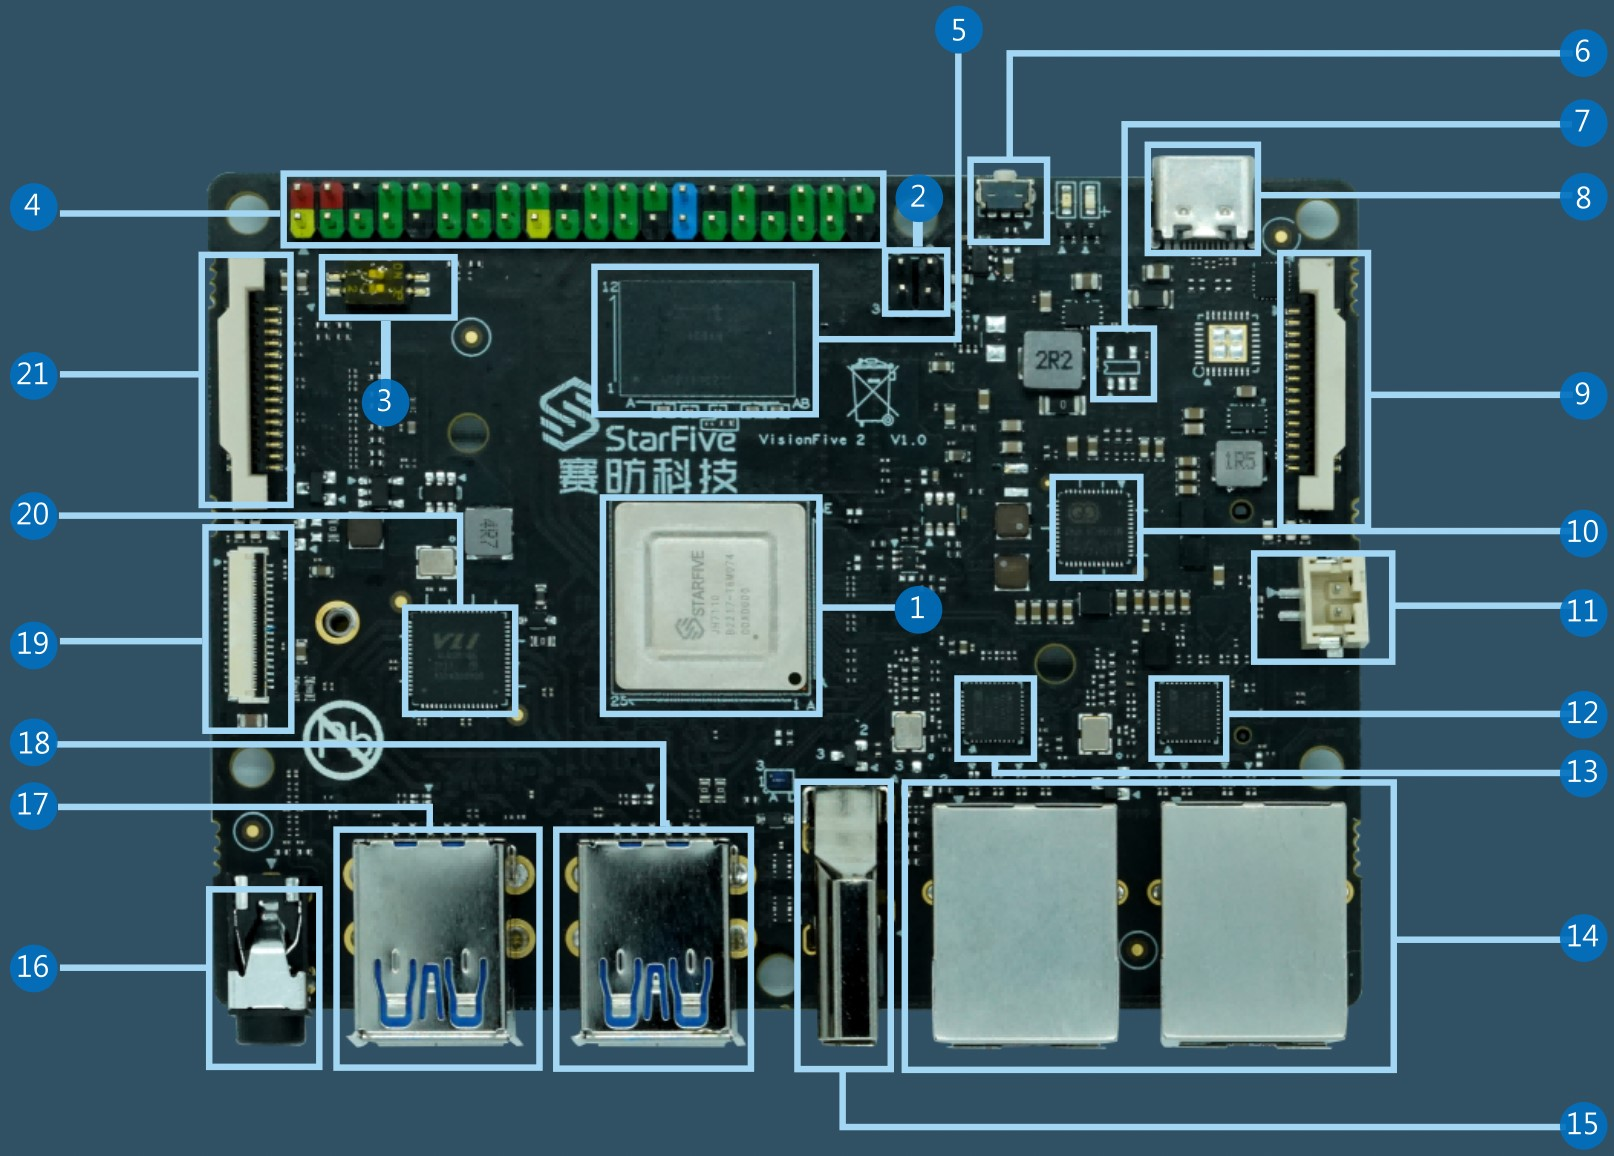
\includegraphics[width=0.58\linewidth]{figures/08-02-赛昉结构.jpg}
	
	
	\raggedright
	\setlength{\parindent}{2em}
	
	连接好后如下图所示
	
	\centering
	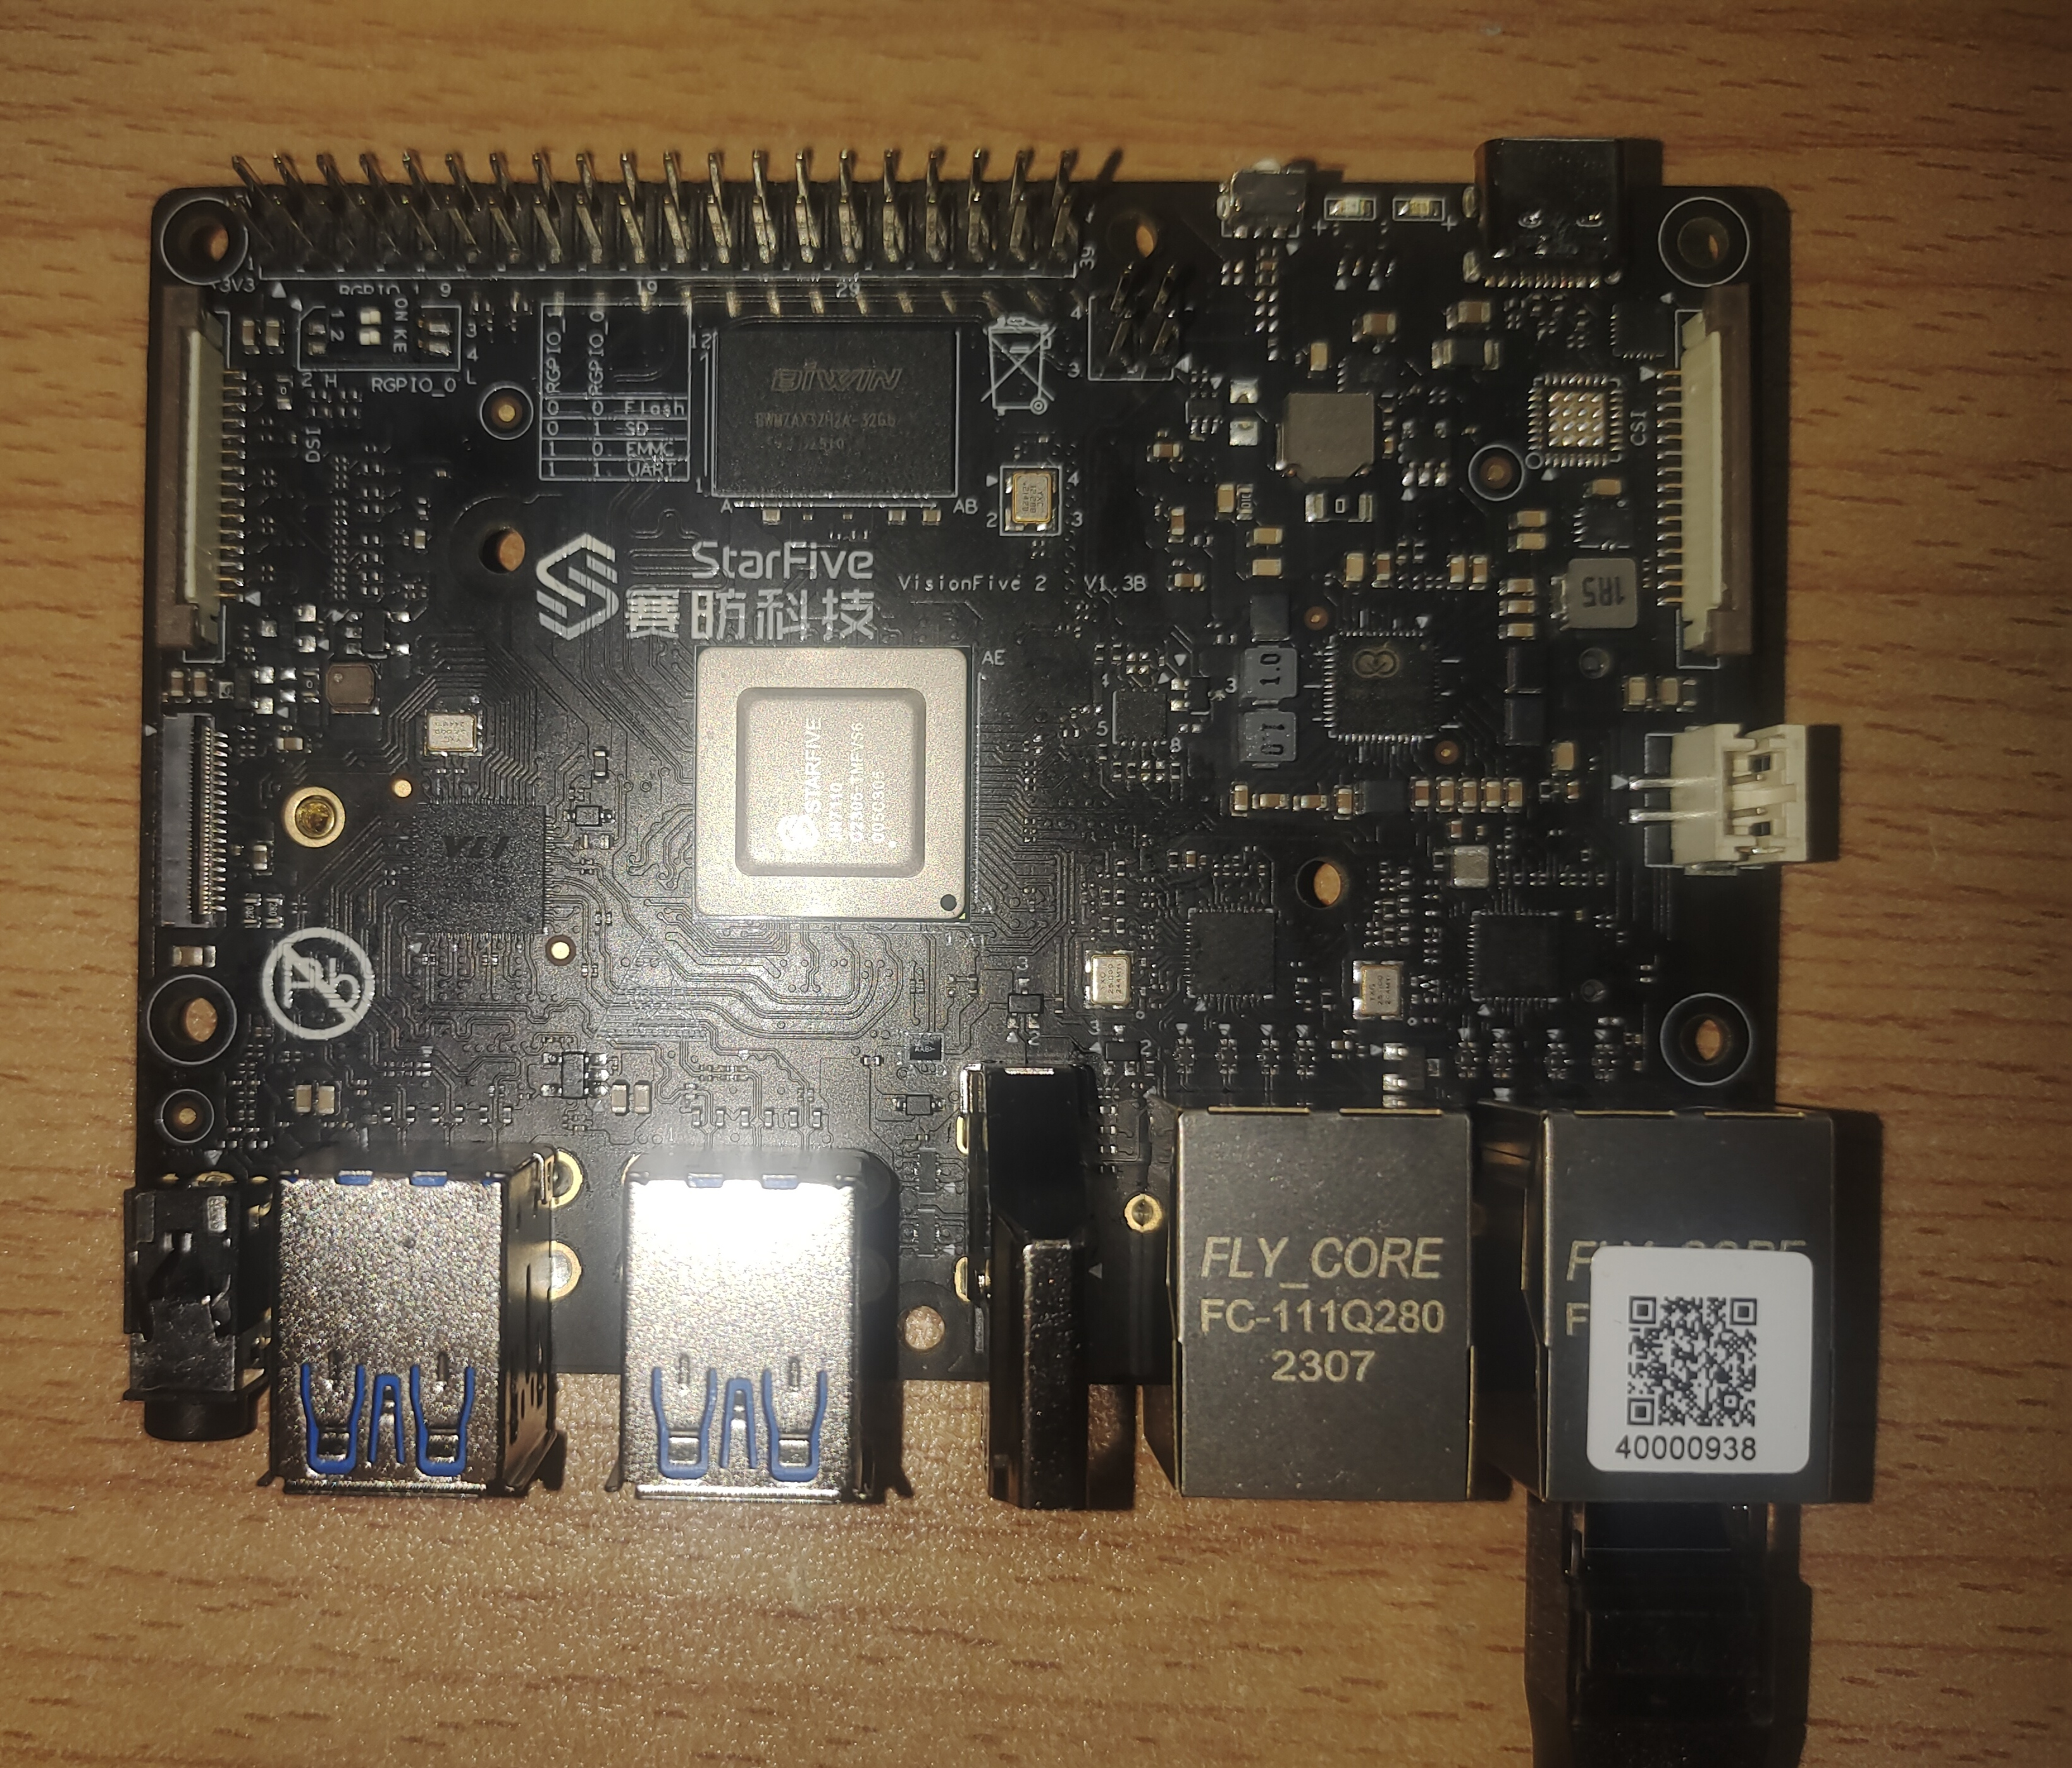
\includegraphics[width=0.58\linewidth]{figures/08-02-连接网线.jpg}
	
}

至此连接完毕,接下来只需将拓展坞连接到电脑即可将开发板连接到电脑,实现插拔方便快捷。

\begin{figure}[htb]
	\centering
	\includegraphics[width=0.58\textwidth]{figures/08-02-连接完毕总览.jpg}
	\caption{
		连接完毕全貌
	}
	\label{fig:pipe}
\end{figure}


\subsection{面向RISC-V64的开发环境搭建与内核运行}
{
\begin{enumerate}
	\item \textbf{编译操作系统内核}
	
	从github上获取NPUcore源码后,使用make命令可以编译内核。编译完成后,会生成os.bin文件,这个便是烧入开发板的内核镜像。由于NPUcore直接使用的是risc-v64的交叉编译工具,该操作可以直接生成risc-v64内核。
	
	\item \textbf{串口连接开发板}
	
	目前使用的星光二号开发板需要使用串口实现交互。可使用的串口工具种类较多,这里以windows操作系统为例,使用
	MobaXterm 工具连接串口。
	
	首先将连接好的开发板插入电脑,开发板指示灯亮起(红色),串口转化器指示灯亮起(红色常亮,有蓝色灯闪烁),说明连接正常。
	~~
	
	\centering
	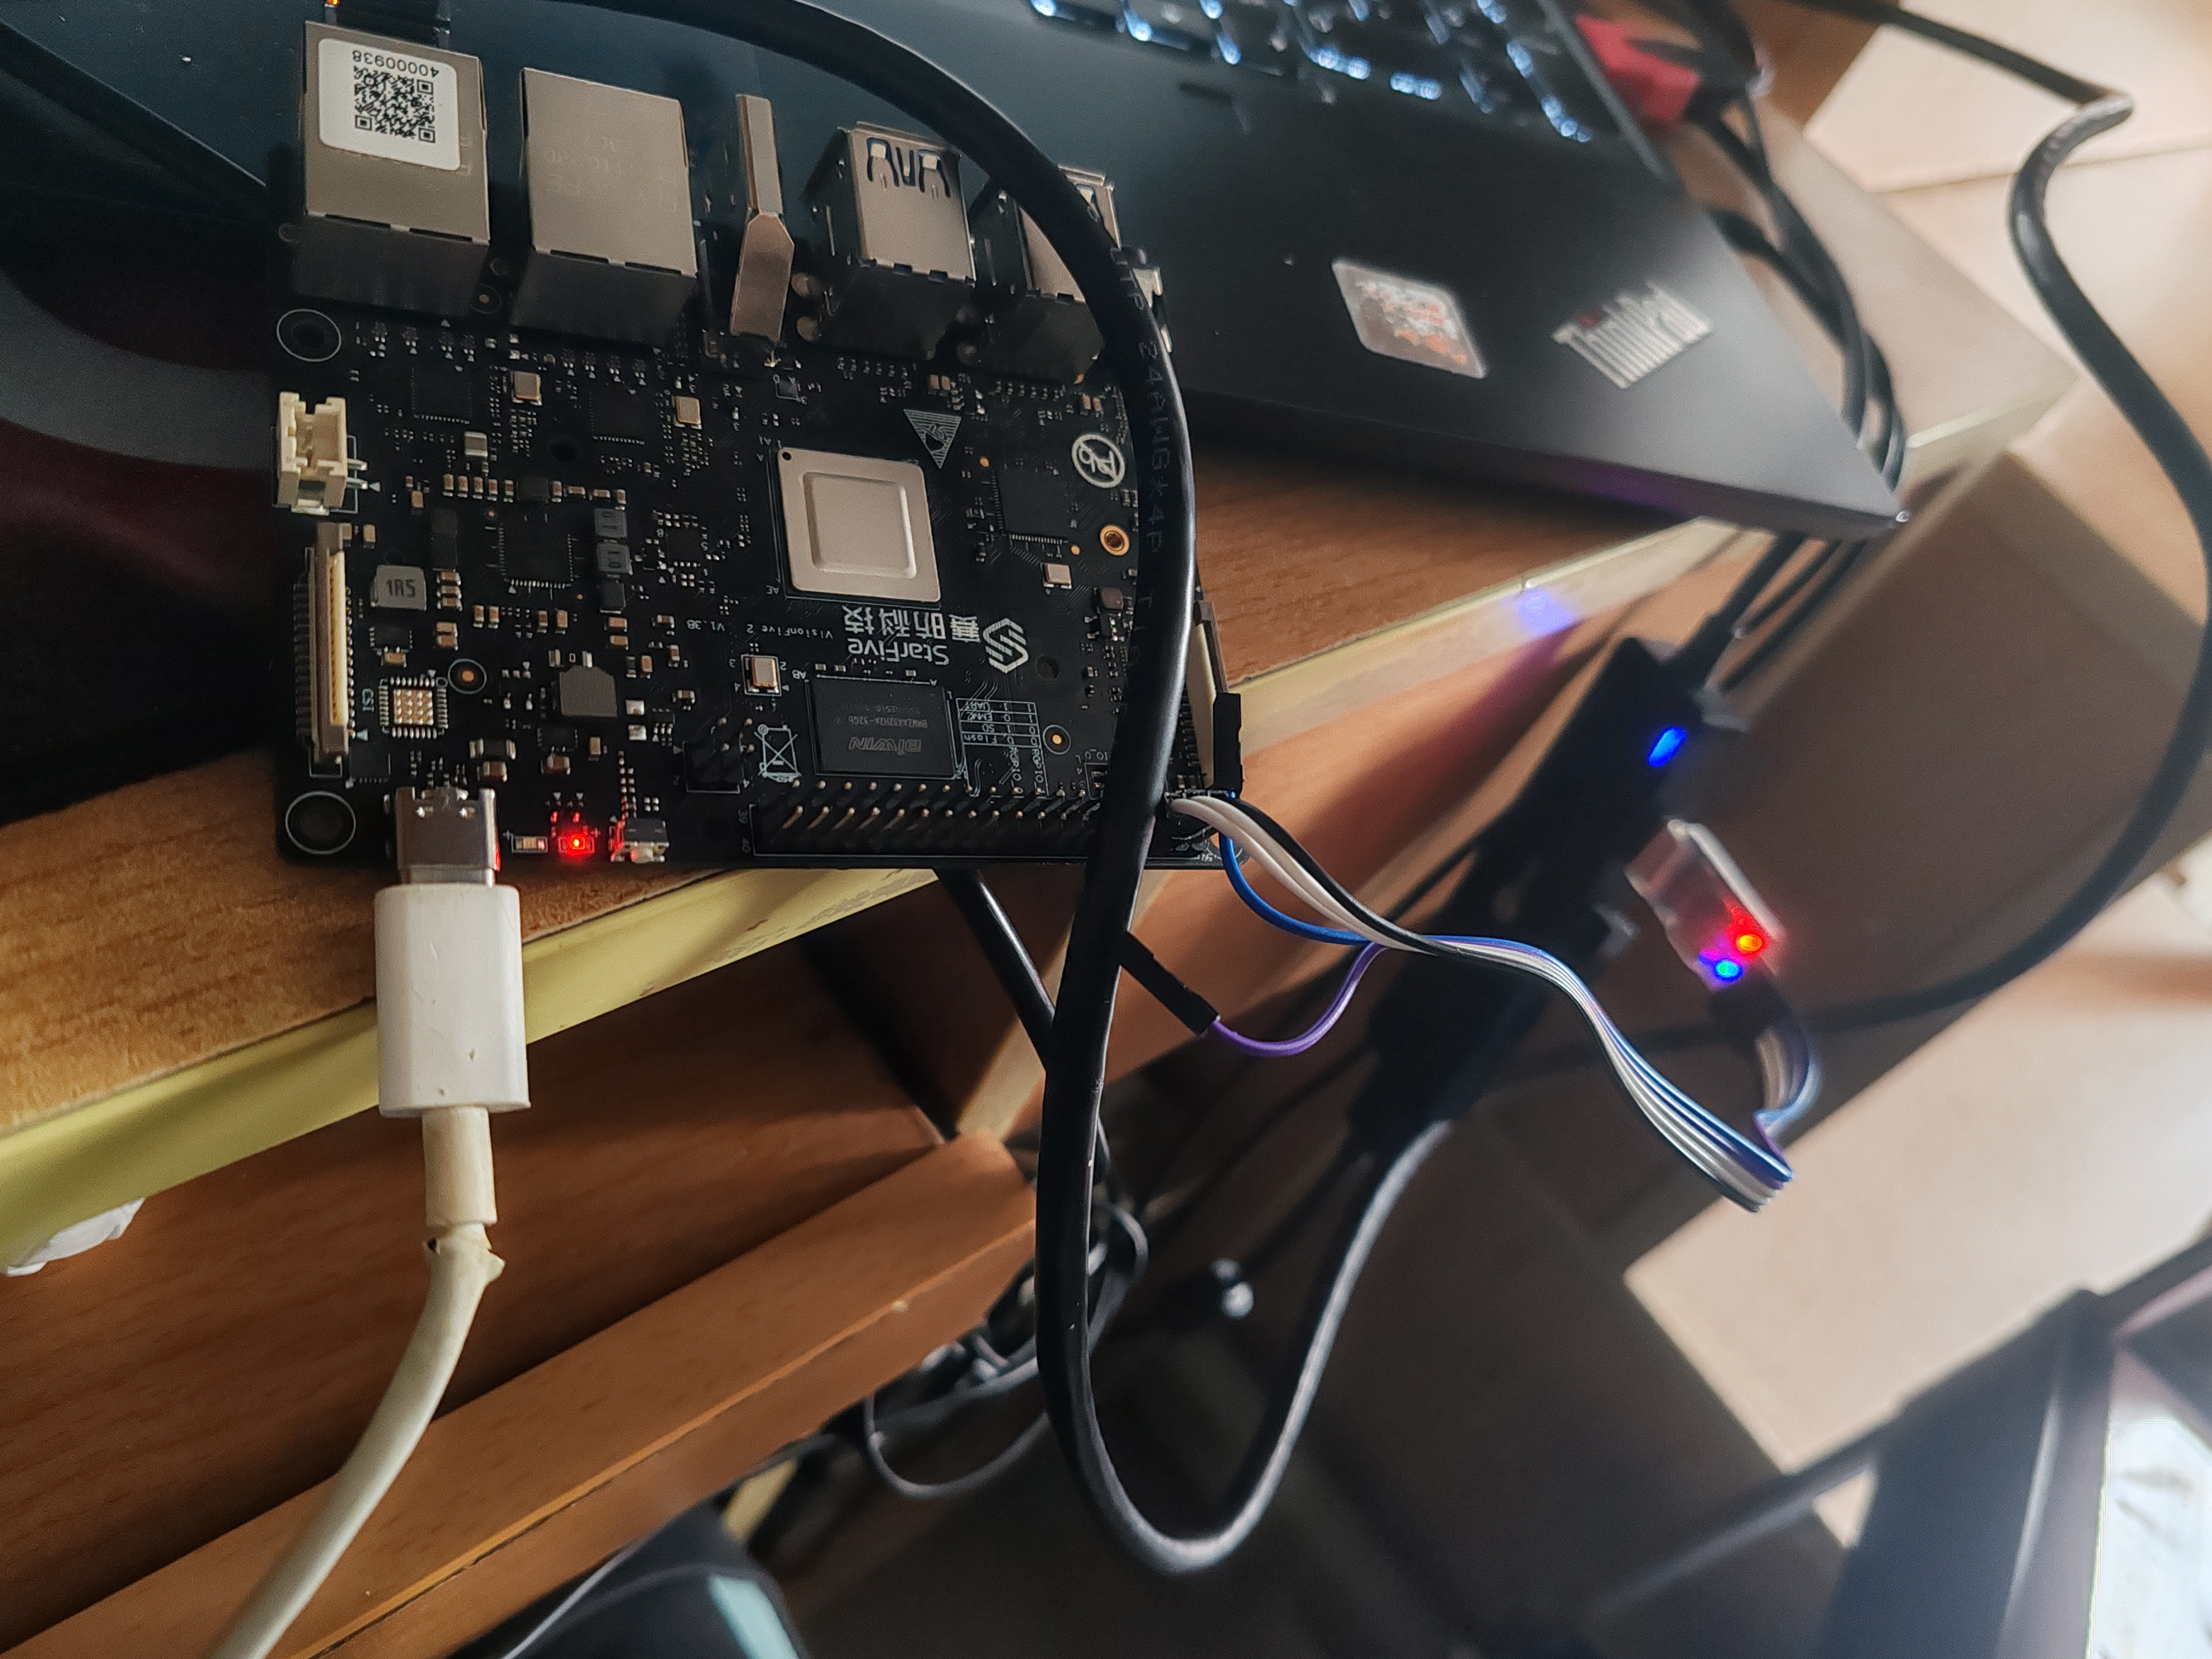
\includegraphics[width=0.58\linewidth]{figures/08-02-星光二号线路.jpg}
	\raggedright
	
	
	打开MobaXterm软件,显示界面如下图:
	
	\centering
	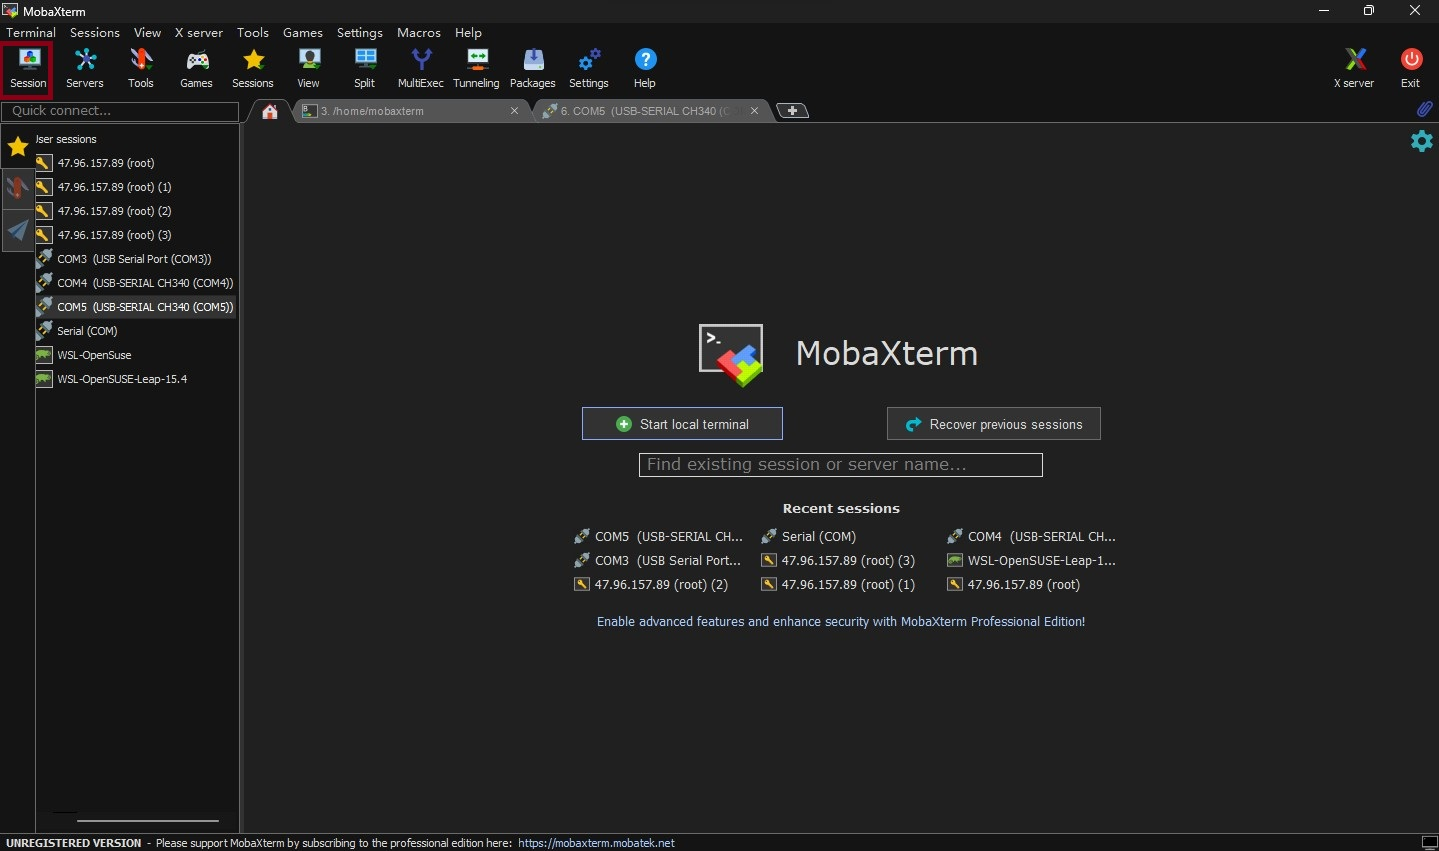
\includegraphics[width=0.58\linewidth]{figures/08-02-MobaXterm界面.jpg}
	\raggedright
	
	点击左上角session:
	
	\centering
	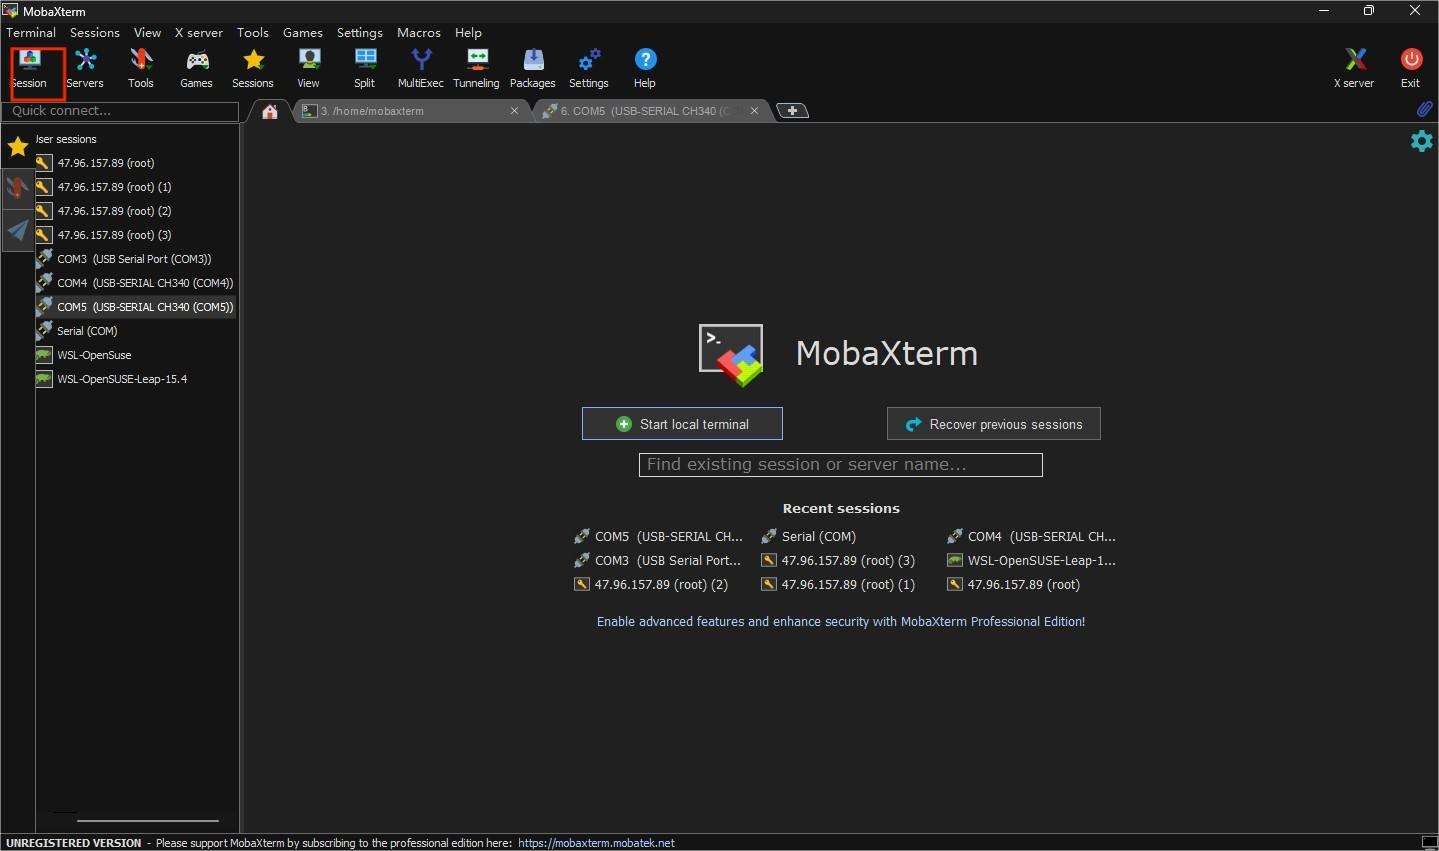
\includegraphics[width=0.58\linewidth]{figures/08-02-session.jpg}
	\raggedright
	
	弹出的窗口中选择“serial”,表示使用新建一个串口会话:
	
	\centering
	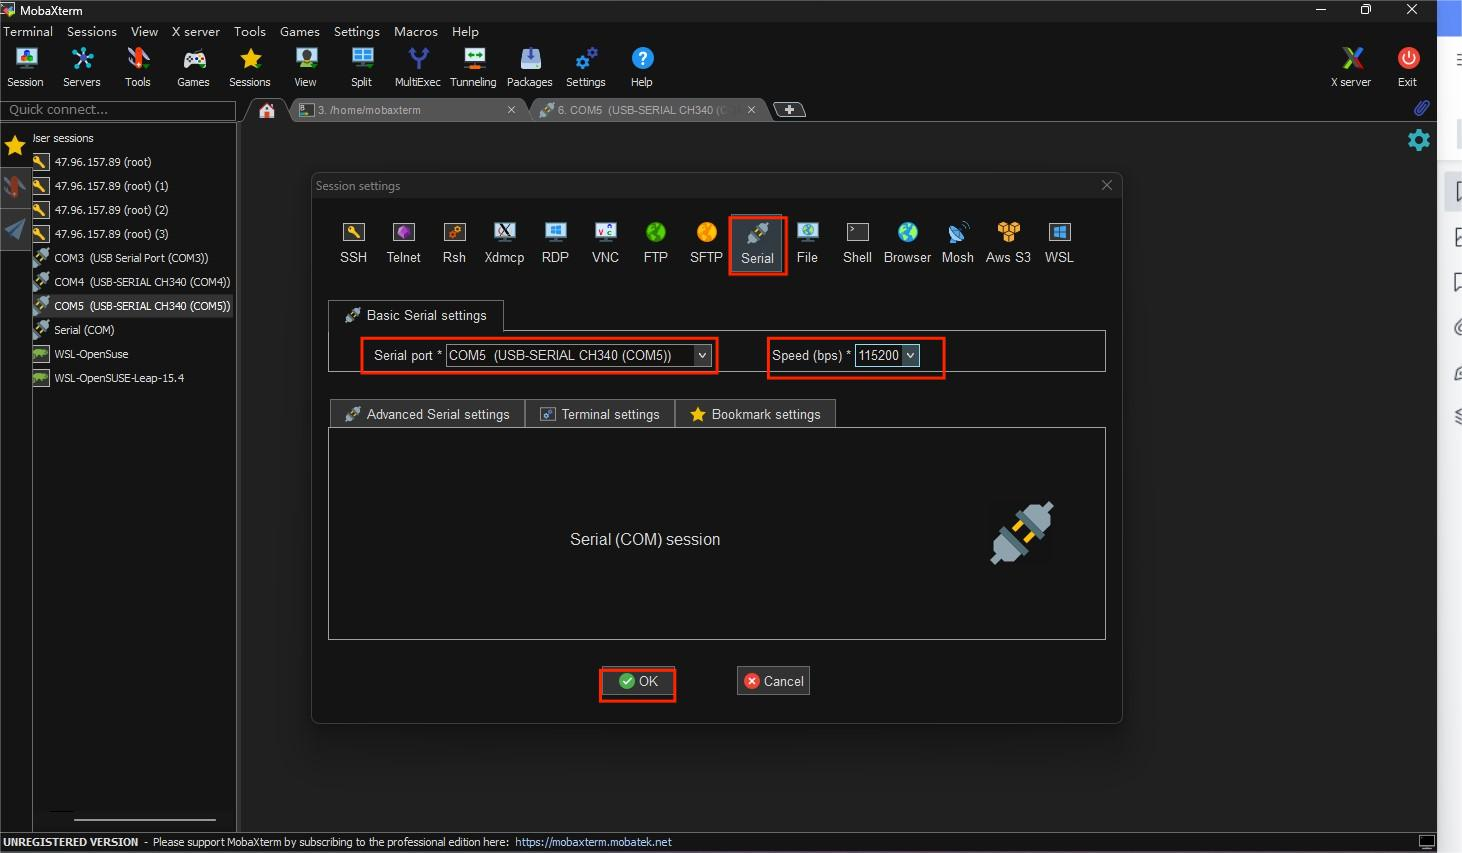
\includegraphics[width=0.58\linewidth]{figures/08-02-串口设置.jpg}
	\raggedright
	
	
	需要设置串口端口和波特率。这里波特率选择115200bps,端口号在开发板正确连接后会自动识别,选择之后点击OK,进入一个命令行:
	
	\centering
	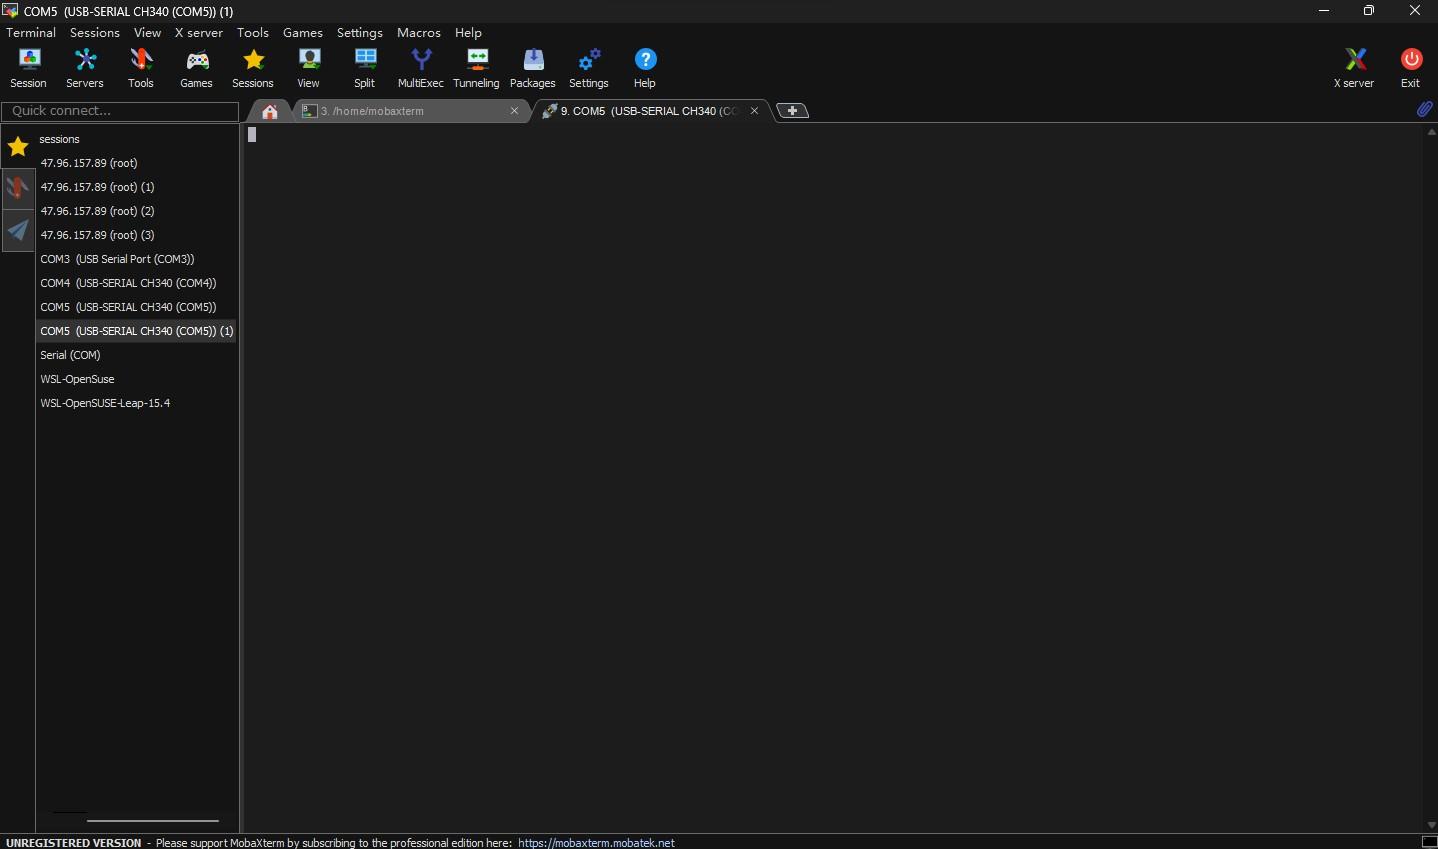
\includegraphics[width=0.58\linewidth]{figures/08-02-串口命令行.jpg}
	\raggedright
	
	切换为英文输入法,输入任意字符,回车,观察到开发板终端的输出:
	
	\centering
	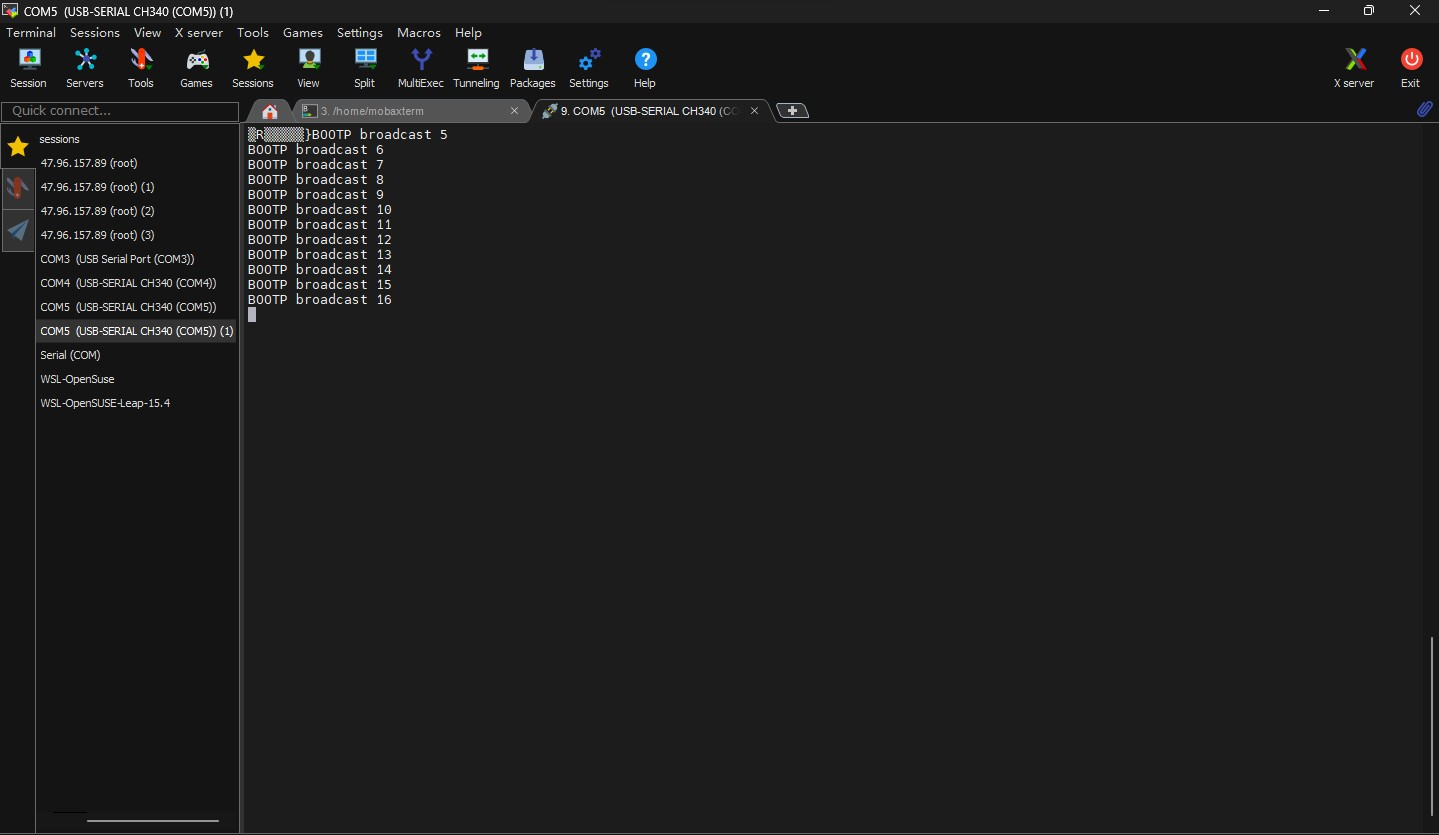
\includegraphics[width=0.58\linewidth]{figures/08-02-串口输出.jpg}
	\raggedright
	
	此时开发板和终端已通过串口连接,终端可以使用命令与开发板进行交互。
	
	\item \textbf{使用tftp协议传输内核镜像}
	
	由于串口用于交互,所以需要通过tftp网络传输内核到开发板。同样tftp网络可以使用多种软件搭建,这里由于
	MobaXterm支持tftp功能,故用MobaXterm举例如何搭建tftp服务器以及如何传输内核文件。
	
	保持串口界面,点击界面左上角的“Server”选项,弹出如下窗口:
	
	\centering
	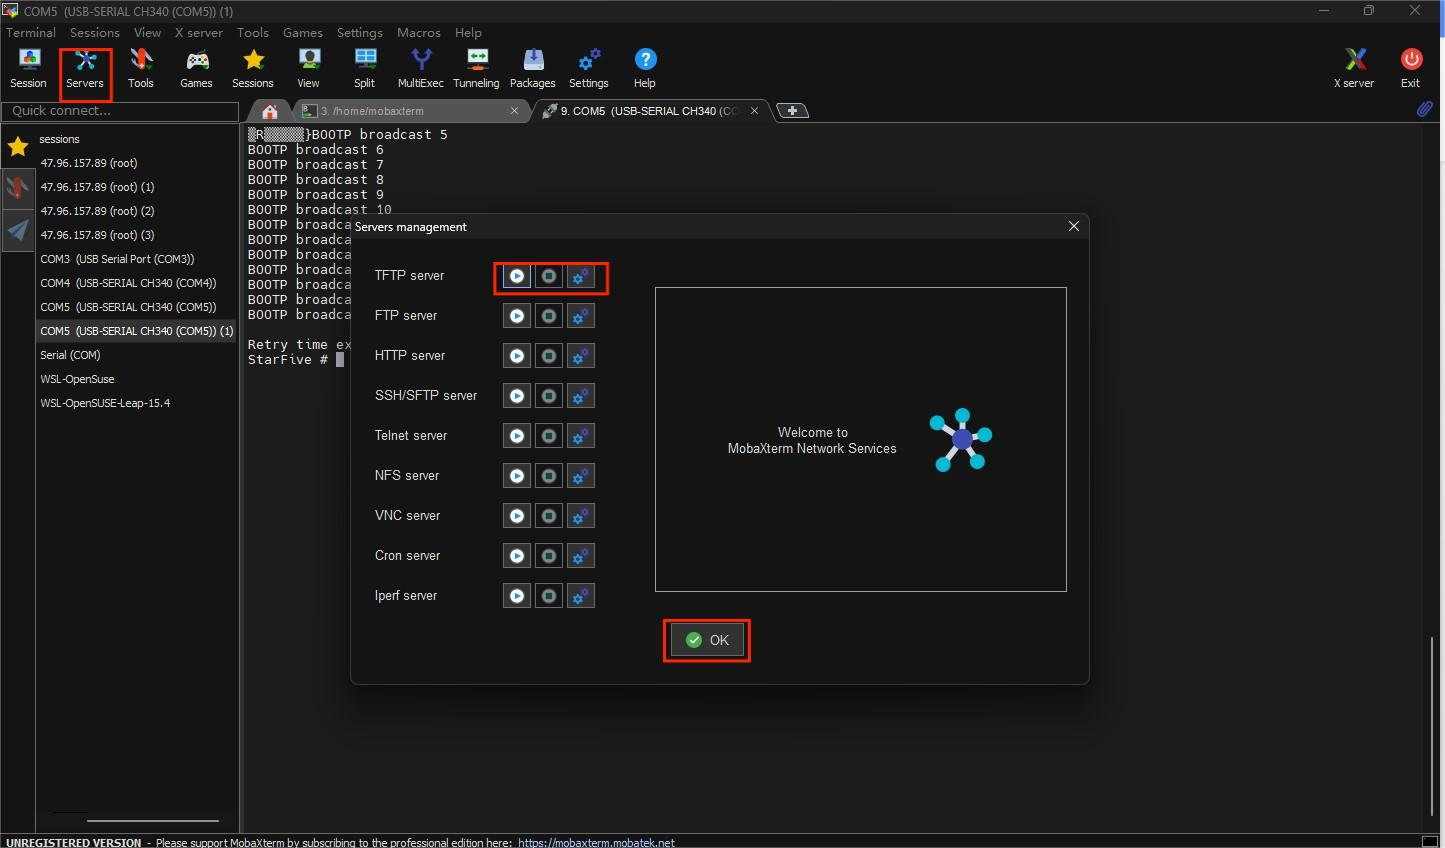
\includegraphics[width=0.58\linewidth]{figures/08-02-tftp服务器搭建.jpg}
	\raggedright
	
	在右方“Root directory”可以设置tftp服务器根地址,也就是开发板可以访问到的目录路径。左上角点击运行按钮可以运行tftp服务:
	
	这时tftp服务器搭建成功,但是需要设置IP地址,将开发板和服务器设置为相同子网,才可以使用tftp服务。
	
	如果终端使用的是自动获取IP地址,则可以通过以下命令查看IP地址:
	
	ifconfig
	
	如果使用的是手动设置的IP地址,以上方法也可以查看。如果需要检查连通性,可使用ping命令,例如如果查到终端IP地址为168.254.242.234,则可以使用如下命令:
	
	ping 168.254.242.234
	
	在“StarFive \#”终端提示符下,输入以下命令设置开发板IP地址:
	
	setenv ipaddr 168.254.242.233
	
	此处需要和终端IP地址不同但是需要和终端IP在同一个局域网中。
	
	执行以下命令设置服务器IP地址:
	
	setenv serverip 168.254.242.234
	
	确认os.bin已经在tftp服务器根目录下,并且tftp服务是打开状态,输入下面命令:
	
	tftpboot 0x80200000 os.bin
	
	便可以将内核镜像下载到开发板上,并设置起始地址为0x80200000。正常执行结果如下:
	
	\item \textbf{运行内核}
	
	上述过程已经将内核镜像下载到开发板上,而且设置了起始地址为0x80200000。接下来输入以下命令便可以开始运行内核:
	
	go 0x80200000
	
	运行结果如下:
	
	
	\centering
	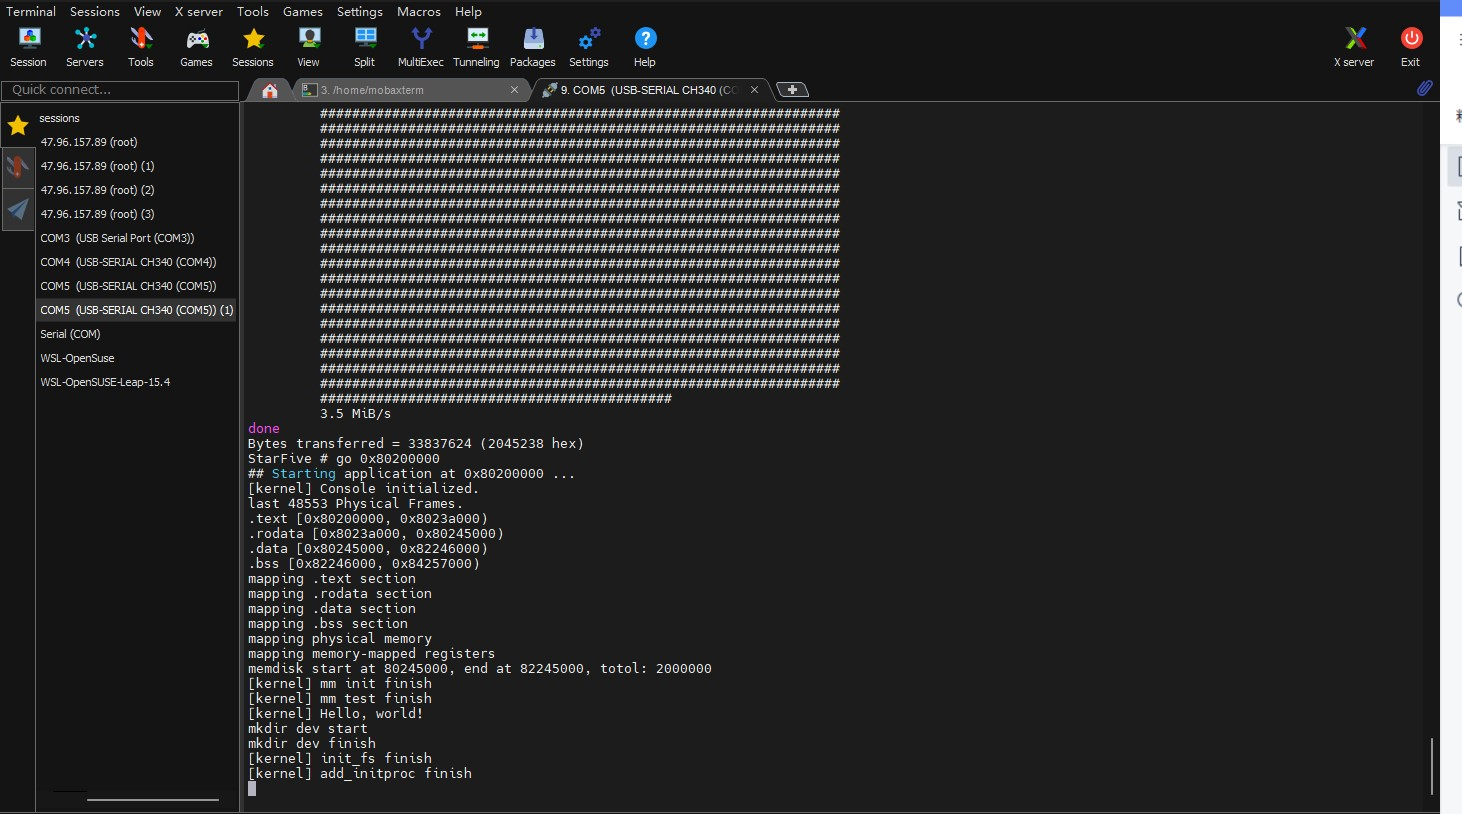
\includegraphics[width=0.58\linewidth]{figures/08-02-内核运行.jpg}
	\raggedright
	
	自此内核启动完成。
	
	
	
	
\end{enumerate}
}